\documentclass[11pt]{article}
\usepackage[margin=1in]{geometry}
\usepackage[T1]{fontenc}
\usepackage[utf8]{inputenc}
\usepackage{lmodern}
\usepackage{amsmath}
\usepackage{booktabs}
\usepackage{graphicx}
\usepackage{caption}
\usepackage{enumitem}
\PassOptionsToPackage{hyphens}{url}
\usepackage[hidelinks]{hyperref}
\usepackage{microtype}

\title{A Seed That Grows by Testing Its Own Changes:\\ A Self-Contained Account for Readers\\ With No Background in the Field}
\author{Maureese Williams}
\date{October 12, 2026}

\begin{document}
\maketitle

\begin{abstract}
This paper describes a computer program that gets better at solving a kind of puzzle over time, and that keeps a change to itself only after that change has passed a strict test. The program is called a \emph{seed agent}, because it is meant to be the thing that grows. Its rules for learning never change. What changes is what it carries from one round of experience to the next: a record of its own past guesses, a model of which puzzle ingredients tend to appear together, and the set of building blocks from which it assembles answers. Every proposed change is tried against the current version on puzzles that neither version has seen, and kept only when the improvement is large enough that luck is an unlikely explanation. The paper assumes no background in machine learning, statistics or programming. Every technical term is defined where it first appears and again in a glossary at the end. The results, in brief: on puzzle sets never used to decide anything, the main development agent's solving rate in its first puzzle setting rose from 17.1\% to 28.8\% over twelve rounds of experience, and it improved in four further settings with different hidden structure. A confirmation procedure that was fixed in advance, with four pass-or-fail conditions and a written forecast, was then run on nineteen fresh random seeds across ten versions. All 89 agent-and-setting pairs of those sealed runs improved, every one of their 171 accepted changes was reproduced exactly by an independent replay, and three of the ten versions passed all four conditions on both of their seeds, at three, six and seven settings. The paper also records what went wrong along the way, because each failure changed the design, and that record is as much the result as the growth is.
\end{abstract}

\section{What this paper is about}

Most programs that learn have two parts. One part is the \emph{procedure}: the fixed rules that say how to turn experience into knowledge. The other part is the \emph{state}: the knowledge itself, which the procedure reads and writes. A cook who follows the same method for learning new dishes, but whose notebook, pantry and sense of which ingredients go together all improve over the years, is improving state while keeping procedure fixed.

This paper studies a program of that kind. Its procedures for learning are fixed code that never changes while it runs. Its state is everything it carries between rounds of experience. The question is whether one program can improve its own state in several different puzzle settings, test every proposed improvement before keeping it, and carry what it keeps into settings with different hidden structure without damaging what it already learned.

The question is worth asking because carried improvements are not automatically safe. A change that helps in one setting can quietly hurt another, and a change that looks like an improvement on a small sample can be luck. Both of these happened in this work, and both led to changes in how the program tests itself. The paper is as much about the testing as about the growth.

A word on terms before anything else. In this research programme, \emph{recursive self-improvement} means a system producing a successor whose learning procedure is better than its own. That is not what happens here. Here the state improves and the procedure does not. The programme's own definition is therefore not met, and the paper says so plainly in Section~\ref{sec:shows}.

The word \emph{seed} has two meanings in what follows, and the paper keeps them apart. A \emph{seed agent} is the program plus its carried state. A \emph{random seed} is a number, such as 644101, that fixes the sequence of pseudorandom choices a run makes, so that the same run can be repeated exactly. Section~\ref{sec:trust} explains why that matters.

\paragraph{What came before.} Three forms of growth had each been shown separately in this programme, in separate programs. First, a program that keeps the building blocks of whatever answer it submits, right or wrong, raised its own solving rate four to ten times across a hundred puzzles, and being told whether it was right added nothing. Second, a grouping of building blocks learned without any labels from 1,600 puzzle worlds let the same program solve 6,993 and 8,077 more puzzles over 18 budget settings than a grouping learned from 400 worlds, on random seeds fixed in advance, with the result independently checked. Third, in a small language for transforming text, a program that built new building blocks out of its failures solved 20 of 24 puzzles where its fixed vocabulary solved 5, on two random seeds. This paper puts the three forms into one program and asks whether they can be carried together.

\section{The puzzles, from scratch}
\label{sec:puzzles}

\subsection{Characters, codes and rules}

The puzzles are about characters. A \emph{character} here is one of 256 symbols, each identified by a whole number from 0 to 255 called its \emph{code}. The letter A, for instance, has code 65. A \emph{rule} is a yes-or-no question about a character, such as ``is its code below 128?'' Every rule can be written as a table with 256 rows, one per character, saying yes or no.

Some rules are easiest to state using \emph{bits}. A code written in binary is a string of eight digits, each 0 or 1, numbered from 0 on the right to 7 on the left. ``Bit 7 is 0'' and ``the code is below 128'' are the same rule, because bit 7 is 1 exactly when the code is 128 or more.

\subsection{What one puzzle looks like}

Each puzzle, called a \emph{task}, hides one rule. The agent is shown a few example strings, and for each string it is shown how long the answer is: the answer is the longest run of characters from the start of the string that all satisfy the hidden rule. The agent's job is to find a rule that fits every example. It then submits that rule. A separate set of \emph{hidden} examples, which the agent never sees, decides whether the submitted rule is actually right.

Here is one task from the implementation. The hidden rule is ``bit 7 of the code is 0''. The agent sees eight examples, of which the first three are:

\begin{center}
\begin{tabular}{ll}
\toprule
answer prefix & rest of the string \\
\midrule
119, 115, 48, 47, 121 & 152, 242, 205 \\
23, 10, 101 & 168, 131, 144, 143, 137 \\
61, 7, 118 & 240, 178, 187, 203 \\
\bottomrule
\end{tabular}
\end{center}

Every character in each answer prefix has a code below 128, and the first character after each prefix has a code of 128 or more. A candidate rule is \emph{consistent} with an example when every character of the answer prefix satisfies it and the first character after the prefix does not.

\subsection{The catalog and the budget}

The agent does not invent rules from nothing. It holds a \emph{catalog}: a long list of candidate rules built from its building blocks, which are described below. At the start of this work the catalog has 82,758 candidate rules. Of these, 77 are consistent with all eight visible examples of the task above, and 17 of those 77 also give the right answer on all sixteen hidden examples.

The agent cannot look at all 82,758 rules for each task. It has a \emph{scan budget}, 1,024 rules per task throughout this paper, and it looks only at the first 1,024 rules in its current ordering of the catalog. The order is the thing the agent learns to improve. Looking at one candidate rule is called a \emph{scan}.

In the task above, scanning the catalog in its starting order, the agent met exactly one consistent rule within its 1,024: ``the code is below 144''. It submitted that rule. The rule fails on a hidden example, so the task counts as unsolved. The agent is not told this. The right rule, ``bit 7 is 0'', was in the catalog all along, but outside the 1,024 rules inspected.

Because the agent found exactly one consistent rule in its window, this submission is what the paper calls a \emph{confident pick}. A confident pick is not a guarantee. On average such picks are right about 90\% of the time, and this one was wrong. Confident picks matter because the agent trusts them more when it learns from its own history.

\subsection{Building blocks: atoms, families and the language}

The smallest building block is an \emph{atom}: one simple yes-or-no rule about a character, such as ``bit 7 is 0'' or ``the code is below 144''. There are 313 atoms in all, in 9 \emph{families} named for the arithmetic operation they use. Examples of families are \emph{bit} (a particular bit is 0 or 1), \emph{threshold} (the code is below some number), \emph{divmod} (the remainder on dividing the code by some number), \emph{gcd} (the greatest common divisor of the code and some number), \emph{popcount} (how many bits of the code are 1) and \emph{xormod} (a combination of bit mixing and remainders).

The set of atoms the agent currently holds is called its \emph{language}. This is not a natural language; it is a vocabulary of rules. The agent starts with 260 of the 313 atoms. Two whole families, popcount and xormod, are withheld. This is deliberate: it creates puzzles whose rules the agent cannot express at all until it invents the missing atoms.

The catalog is built from the language. It contains every atom, the opposite of every atom (its \emph{complement}: ``bit 7 is 1'' is the complement of ``bit 7 is 0''), and every pair of atoms from different families joined by \emph{and} (both must hold), \emph{or} (at least one must hold) and \emph{xor} (exactly one must hold). Rules that behave identically on all 256 characters are merged into one row. From the starting 260 atoms this gives 82,758 rows; from all 313 atoms it would give 166,596. Whenever the language changes, the catalog is rebuilt.

\subsection{Two different ways to fail}

The agent can fail a task for two different reasons, and the distinction organises the whole design.

\begin{enumerate}[leftmargin=*]
\item The right rule is in the catalog but outside the budgeted window. The worked example above is this kind of failure. The remedy is a better ordering of the catalog, so that the right rules come earlier. The paper calls this \emph{search guidance}.
\item The right rule cannot be built from the current language at all. A task whose hidden rule uses a popcount atom is this kind of failure for the starting agent. The remedy is to add the missing atom. The paper calls this \emph{invention} or \emph{extending the language}. In some puzzle worlds a third of the rules cannot be expressed by the starting language.
\end{enumerate}

Two cautions. A task on which the agent finds no consistent rule does not prove that an atom is missing; it means only that the budgeted search found none. And invention here is not unrestricted creativity: the agent assembles candidate atoms from a small fixed grammar of arithmetic expressions, described in Section~\ref{sec:ops}.

\section{How the puzzles are organised: worlds, areas, pools and lives}
\label{sec:areas}

\paragraph{Worlds.} Tasks do not come one at a time from nowhere. A \emph{world} is a hidden set of 14 atoms, and every task in that world has a rule built only from those 14. A world has 100 tasks. The tasks of a world are therefore related, as dishes from the same pantry are related, and an agent that notices which atoms a world uses can order its catalog to favour rules built from them. Think of a world as a cuisine, its 14 atoms as its pantry, and each task as a dish.

\paragraph{Areas.} An \emph{area} is a recipe for generating worlds, with a particular hidden structure deciding which atoms go together. Four kinds of area are used. Their names in the code are given in parentheses.

\begin{itemize}[leftmargin=*]
\item \textbf{Mechanism worlds} (\texttt{mech}). A world draws three of seven atom families and takes its 14 atoms from those three. The agent's starting language lacks the two remaining families, so a world that uses one of them contains rules the agent cannot express. A fifth of the possible family triples are withheld from the agent's experience as \emph{untrained combinations}; they appear only in evaluation. The agent's experience draws three quarters of its worlds from trained triples and a quarter from triples that include a family the language lacks.
\item \textbf{Drawn partitions} (\texttt{drawn7}, \texttt{drawn11}, \texttt{drawn13}). Every atom of every family is assigned at random to one of a few groups, with no regard for family. A world picks some groups and draws its 14 atoms from them, and each atom has some chance to \emph{slip} to a random atom instead. Because the grouping cuts across families, nothing the agent learned about mechanism worlds helps here except its language. The three areas differ in structure: 9 groups with 3 per world and a slip chance of 0.15; 12 groups with 4 per world and no slip; 6 groups with 2 per world and slip 0.15. The agent is never told how many groups a world uses.
\item \textbf{Metric worlds} (\texttt{metric777001}, \texttt{metric555001}). Each atom is given a numerical fingerprint describing how its yes-or-no answers are distributed across the 256 characters. A hidden weighting over the parts of that fingerprint is drawn once and shown to nobody. A world is one centre atom together with the 13 atoms whose fingerprints are nearest to it under the hidden weighting. Here the hidden structure is about how atoms behave, not how they are written. A quarter of each round's worlds are centred on an atom of the two withheld families. The two areas use two different hidden weightings.
\item \textbf{String tasks} (\texttt{str7}). A different kind of puzzle entirely, added late in the work to test whether the agent's machinery depends on the character puzzles. A task is three visible and six hidden pairs of an input string and an output string, produced by a hidden small program. A program glues together up to three pieces; each piece is either the part of the input between two positions, optionally changed to upper or lower case, or a fixed constant. The positions, the three case operations and six constants are the building blocks here, called \emph{keys}: 58 in all, from which 9,400 candidate pieces are built. A world is 14 keys from three of seven key families, with 100 tasks over programs that use only those keys. The twelve positions that refer to runs of upper-case or lower-case letters are withheld from the starting language, which therefore has 46 keys and 5,334 pieces. A task is solved when the first program in the agent's budgeted window that reproduces the three visible pairs also reproduces the six hidden ones.
\end{itemize}

\paragraph{Pools.} Within an area, worlds fall into \emph{pools} that the scoring can tell apart but the agent cannot. Mechanism worlds and string tasks have three pools: \emph{trained} (family combinations the agent lives in), \emph{untrained} (combinations withheld from its experience) and \emph{unfamiliar} (a family its starting language lacks). The drawn and metric areas have one pool each. Pools let the evaluation ask whether the agent got better only where it practised, or everywhere.

\paragraph{Lives.} A \emph{life} is one round of experience followed by one round of self-change. In the development runs a life is 48 worlds of one area, 100 tasks each; in the confirmation runs a life is 96 worlds. Only after living all of them does the agent propose changes to itself and test them. Lives in different areas can be interleaved, because the agent saves its state after every step.

\paragraph{What the agent is never told.} It is never told which family an atom belongs to, what a world's true 14 atoms are, which pool a world came from, or whether any particular submission was right. Those labels are used only by the scoring, after the fact.

\section{What the agent carries, and what stays fixed}

The \emph{carried state} is everything the agent keeps from one life to the next:

\begin{itemize}[leftmargin=*]
\item its \textbf{language}, the atoms it currently holds, including any it invented;
\item its \textbf{experience}, one record per world it has lived, naming the area and the atoms behind its confident picks and behind all its picks, stored by atom name so that the records survive changes to the language;
\item for each area, a \textbf{world and self model} and a flag saying whether to build a \textbf{search prior} from that area's experience, both explained in the next section;
\item the list of \textbf{invented atoms} and the life each entered;
\item a \textbf{ledger} recording every proposed change, the test it faced and its outcome;
\item a \textbf{resource account} of everything spent on living, testing and inventing.
\end{itemize}

The language, the experience and the ledger are shared across all areas. The model and the prior belong to one area each. This sharing is where the danger lies: a language change made for one area changes the catalog that every other area's model was fitted over.

The fixed part is the code of the five operations in the next section. Nothing the agent does alters that code. When the acceptance rule changed during this work, the experimenter changed it, and the paper records each change.

\section{The five operations}
\label{sec:ops}

\paragraph{Live: collect evidence while solving related tasks.} The agent draws fresh worlds of an area and works through each as a stream of 100 tasks at the scan budget. Within a world, the atoms of each answer it submits are moved towards the front of its catalog order for the next task, so that a world's own pantry is discovered progressively. Two carried objects reorder the catalog further. The area's model, when there is one, turns the atoms earned so far in the current world into beliefs about which groups of atoms this world uses, and promotes the rows those groups build. The area's prior, when there is one, starts the scan from an order based on how often atoms appeared together in the agent's own earlier worlds of that area, with half of each task's budget reserved for the order the agent would use with no prior at all. With neither, the agent scans in catalog order. It receives no feedback on whether any answer was right.

\paragraph{Reflect: turn accumulated evidence into better search guidance.} After a life, the agent looks back over every world it has lived in that area and fits a \emph{world and self model}. The ``world'' half asks which atoms tend to occur together; the ``self'' half asks how reliably the agent finds each atom when it is present, and how often it mistakenly picks up an atom that is absent. In detail, the model supposes that atoms belong to hidden groups and that each world uses a few groups. It fits, from the agent's confident picks alone, which group each atom belongs to, how often each combination of groups occurs, and for each atom two rates: a \emph{discovery rate}, how often the agent finds the atom when a world contains it, and an \emph{import rate}, how often the agent earns the atom through a wrong pick in a world that does not contain it. The fitting uses a standard iterative method called expectation-maximisation, which alternates between guessing the hidden group labels and re-estimating the rates until the two agree. An atom whose discovery rate falls below 0.10 is filed in no group: the agent meets it only through its own mistakes, and that verdict is used later to clean up the language. The model's size, 6 to 8 groups and 2 to 4 groups per world, is chosen by how well each candidate size predicts the most recent fifth of the agent's worlds in that area. The refit model, together with a prior built from the area's experience, forms one proposed change.

\paragraph{Extend: propose new atoms from the tasks the agent could not cover.} For the third of the life's worlds with the most tasks on which no consistent rule was found, and only those worlds with at least 15 such tasks, the agent enumerates small arithmetic expressions from a fixed grammar, 3,456 candidates distinct up to complement, searched smallest first. Each candidate is tested against the uncovered tasks, alone, complemented, or joined by and, or or xor to one atom the agent earned in that world. A candidate is proposed only if it fits at least two uncovered tasks. The reason is recurrence: an atom a world is actually built from shows up in several of its rules, while a chance fit shows up once. At most 40 atoms are proposed per life. The first version of this operation accepted single fits, and every extension it proposed lost its test.

\paragraph{Prune: propose removing inventions that never paid.} An invented atom is proposed for removal two or more lives after it entered if it has never appeared in a confident pick, or if every area model that has seen it rates it as found only through wrong picks.

\paragraph{Prove: decide whether a change deserves to persist.} This is the operation the whole design turns on. Its name is a misnomer the implementation kept: it is an empirical test, not a mathematical proof, and the paper otherwise says \emph{test} and \emph{accept}. After a life, the agent proposes all three kinds of change at once and tests the combination. If the combination fails, it tests each part on its own. A test works as follows.

\begin{enumerate}[leftmargin=*]
\item A \emph{held-out set} of worlds of the area is drawn for that life. ``Held out'' means the agent never lived these worlds and they are used only for comparison. In the development runs the set has 24 worlds per pool; in the confirmation runs it has at least 48.
\item Both the current state and the candidate state are run on every world of the set, and for each world the difference in tasks solved is recorded. Because the two states are compared on the same worlds, this is a \emph{paired comparison}: world-to-world variation in difficulty cancels out.
\item The per-world differences are summarised by a \emph{95\% bootstrap interval}. The procedure resamples the list of differences with replacement 4,000 times, computes the average of each resample, and reports the range that contains the middle 95\% of those averages. If that whole range lies above zero, the candidate's gain is unlikely to be luck, and it is accepted. If the range includes zero, the data cannot tell a real gain from noise, and the candidate is rejected. A candidate that is clearly behind after the first half of the set is stopped there, to save cost.
\item A candidate that changes the language is also run on a smaller held-out set of every other area the agent has lived in, 12 worlds per pool in development and 24 in confirmation, and is rejected if its total there falls more than 2\% below the current state's. This is the \emph{cross-area check}, added after the failure described in Section~\ref{sec:interference}. A language change is checked only against areas of the same puzzle form, since the character and string forms build their catalogs from disjoint building blocks.
\item From version 10 of the confirmation protocol, a candidate whose interval includes zero but whose average gain is large enough that doubling the sample would be expected to clear zero is run once more on an \emph{extension set}, a second held-out set of the same size drawn fresh, and the decision is made on the two sets together. This was added after the failure described in Section~\ref{sec:noise}.
\item Every world run in any test is charged to the agent's resource account, so that the cost of testing is visible and can be gated.
\end{enumerate}

The agent therefore receives feedback at exactly one point: aggregate scores when it decides which changes to keep. It never receives feedback on individual answers.

\begin{figure}[t]
\centering
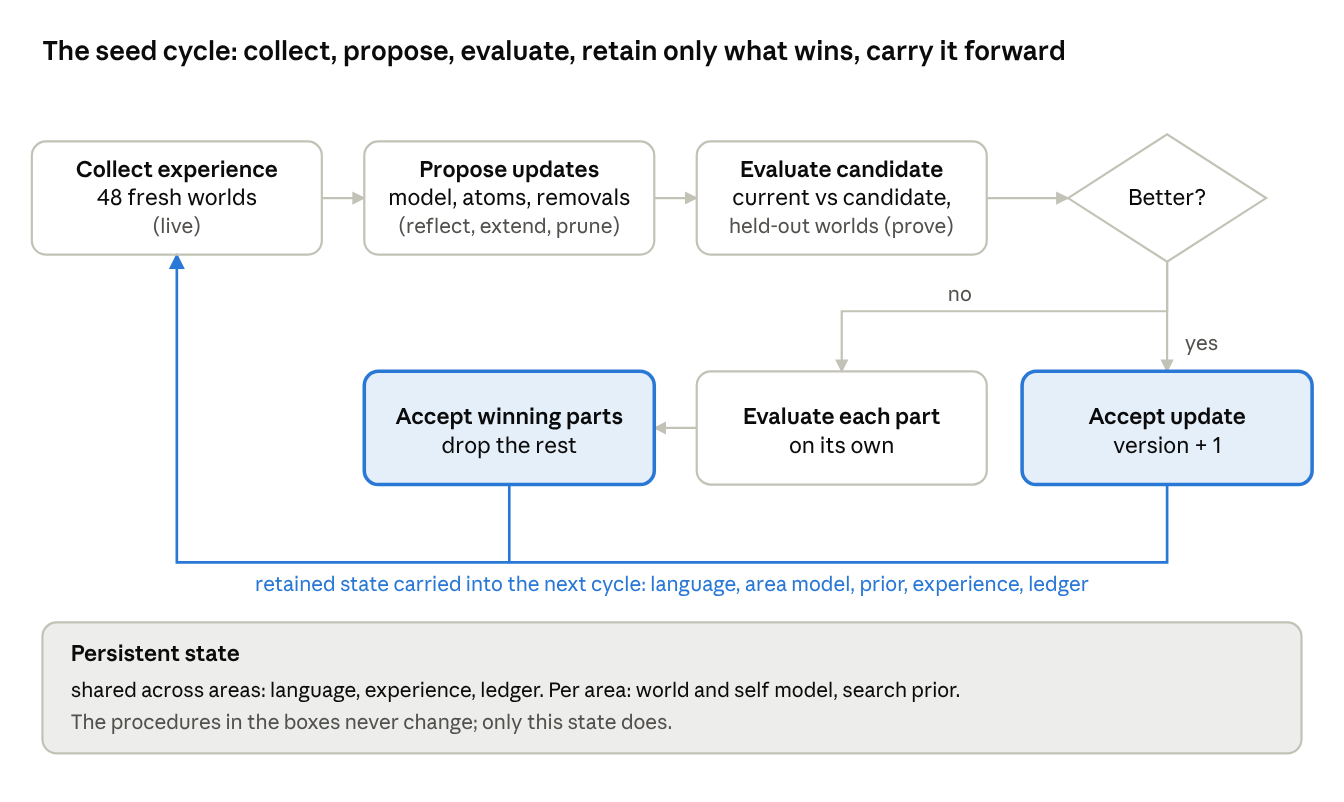
\includegraphics[width=\linewidth]{fig-seed-life.png}
\caption{One life of the seed agent. It collects experience in fresh worlds, proposes changes of three kinds, tests the combined candidate against the current state on held-out worlds drawn for that life, accepts it if it wins and otherwise tests each part alone, and carries the retained state into the next life. The language, experience and ledger are shared across areas; the model and prior belong to an area. Implementation names in parentheses.}
\label{fig:life}
\end{figure}

Figure~\ref{fig:life} shows the cycle. The boxes are the fixed procedures. The state on the return path is what changes.

\section{How the result was made trustworthy}
\label{sec:trust}

A program that improves on the puzzles it was designed against proves little, because the designer may have tuned it to those puzzles. The work was therefore split into two phases with different rules.

\paragraph{Development.} Three agents were run on random seeds 644101, 643101 and 645101, named \texttt{s1}, \texttt{s2} and \texttt{s3}. Their results were inspected as the design changed, and the acceptance rule was revised twice in response to what they showed. These results are informative but not evidence in the strict sense, because the design was adjusted while looking at them.

\paragraph{Confirmation.} Once the design was settled, a protocol was written down and frozen. Freezing means four things.

\begin{itemize}[leftmargin=*]
\item \textbf{The code was hashed.} A \emph{hash} is a short fingerprint computed from a file's exact contents; changing a single character changes the fingerprint. The fingerprints of the source files were recorded, so that anyone can check that the code that ran is the code that was frozen.
\item \textbf{The random seeds were sealed.} A \emph{random seed} is the number that determines every pseudorandom choice a run makes: which worlds are drawn, which held-out sets, which resamples. Running the same code with the same seed reproduces the same run exactly. Sealed seeds, 919100 onward, were chosen in advance and never used before, so the design could not have been tuned to them.
\item \textbf{A forecast was committed.} Before each version ran, the probability that all four gates would pass on both of its seeds was written down. This keeps the experimenter honest about what was expected.
\item \textbf{Four gates were stated in advance.} A \emph{gate} is a pass-or-fail condition. The four are: (1) \emph{growth}, every area's score on a fresh held-out set rises by at least 15\%; (2) \emph{safety}, no pool of any area ends below 90\% of its starting score; (3) \emph{cost}, the worlds spent on testing are at most a stated multiple of the worlds spent living, 2.5 times in the three-area protocol and more when more areas are checked; (4) \emph{audit}, every accepted change is reproduced exactly by an independent replay from the saved state, and no two acceptances in an area used the same held-out set.
\end{itemize}

\paragraph{The final check.} The gates are scored on \emph{fresh} held-out sets: one further set per area, 24 worlds per pool, drawn with a random salt no test ever used. A \emph{salt} is an extra number mixed into the random draw so that a set is distinct from every other. On these sets the starting state (starting language, no model, no prior) and the retained state are run once each, and the two totals are compared. No acceptance decision ever saw these sets.

\paragraph{The audit.} Because every run is determined by its seed, an \emph{auditor} program can rebuild the state the agent had before and after each accepted change, draw the same held-out set, run both states again, and check that the totals and the interval come out identical to what the ledger recorded. If they do, the acceptance ``replays exactly''. This catches bookkeeping errors, and it caught two during the work.

\paragraph{Each version runs on two new seeds.} Every change to the protocol, however small, was frozen as a new version with new hashes and run on two seeds never used before. A version passes only if all four gates pass on both. Table~\ref{tab:evidence} summarises which information each stage of the system is allowed to use.

\begin{table}[h]
\centering
\caption{What information is used where. The final evaluation sets were never used to accept anything.}
\label{tab:evidence}
\small
\begin{tabular}{p{0.18\linewidth}p{0.44\linewidth}p{0.3\linewidth}}
\toprule
Stage & Information used & Decision it supports \\
\midrule
Solving tasks & Visible examples, own submissions, how many consistent rules were in the window & Search order and experience collection; no feedback on correctness \\
Choosing the model's size & How well each size predicts the most recent fifth of the area's lived worlds & Number of groups \\
Accepting a change & Aggregate held-out scores, paired over worlds & Whether a change is kept \\
Final evaluation & Further held-out sets never used for acceptance & The reported gains and the gates \\
\bottomrule
\end{tabular}
\end{table}

\section{Results}

\subsection{Development: did the three agents improve?}

In ten of eleven agent-and-area pairs, yes. Table~\ref{tab:growth} gives the counts on held-out sets never used for acceptance. The main agent \texttt{s1} lived twelve lives in mechanism worlds, four in \texttt{drawn7}, four in metric worlds, three in \texttt{drawn11} and two in \texttt{drawn13}. Its mechanism-world solving rate rose from 17.1\% to 28.8\% (1,232 to 2,072 of 7,200 tasks), with one qualification: trained family combinations rose from 26 to 49 tasks per world and worlds with an unfamiliar family from 5 to 19, but untrained combinations fell from 20.5 to 18.6. Section~\ref{sec:dilution} explains why. Agents \texttt{s2} and \texttt{s3} lived three mechanism lives and two lives each in \texttt{drawn7} and metric worlds.

The one exception is \texttt{s3} in the drawn partition, where the retained state scored 246 against a start of 280. The loss came from a 40-atom language extension accepted in metric worlds, which passed its cross-area check on the drawn partition on a 12-world set (124 to 148) and then lost on the larger 24-world evaluation set. The lesson, taken into the confirmation protocol, is that a 12-world check is too small.

\begin{table}[t]
\centering
\caption{Development agents: tasks solved on held-out sets never used by an acceptance test, 24 worlds per pool, scan budget 1,024.}
\label{tab:growth}
\begin{tabular}{llrrr}
\toprule
Agent (random seed) & Area (lives) & Start & Retained & Tasks \\
\midrule
s1 (644101) & mechanism worlds (12) & 1,232 & 2,072 & 7,200 \\
s1 & drawn7, 9 groups of 3 (4) & 211 & 364 & 2,400 \\
s1 & metric worlds (4) & 427 & 2,076 & 4,800 \\
s1 & drawn11, 12 groups of 4 (3) & 199 & 360 & 2,400 \\
s1 & drawn13, 6 groups of 2 (2) & 294 & 442 & 2,400 \\
s2 (643101) & mechanism worlds (3) & 1,292 & 1,879 & 7,200 \\
s2 & drawn7 (2) & 221 & 424 & 2,400 \\
s2 & metric worlds (2) & 492 & 1,520 & 4,800 \\
s3 (645101) & mechanism worlds (3) & 1,081 & 2,074 & 7,200 \\
s3 & drawn7 (2) & 280 & 246 & 2,400 \\
s3 & metric worlds (2) & 394 & 1,349 & 4,800 \\
\bottomrule
\end{tabular}
\end{table}

\paragraph{Which kinds of change were kept.} Refit models were the most consistently accepted: on \texttt{s1} a refit model was accepted on every mechanism life from 0 to 6 and on the first life of every other area, and on \texttt{s2} and \texttt{s3} on all three mechanism lives. Language extensions were accepted less often, 6 of 24 proposed on \texttt{s1}, and every extension proposed on \texttt{s2} and \texttt{s3} in mechanism worlds was rejected. Four removals were accepted on \texttt{s1}, taking out 23, 26, 25 and 55 invented atoms. Over its 26 versions, \texttt{s1} accepted 16 models, 6 extensions and 4 removals, and rejected 18 extensions, 6 models and 1 removal. These are counts of decisions, not a breakdown of where the gain came from: the measurements do not separate what invention contributed from what better search contributed.

\paragraph{What was invented.} At its 26th version, \texttt{s1}'s language held 111 invented atoms. Of these, 26 reproduce true popcount atoms and 29 true xormod atoms, the two withheld families, and 56 behave like nothing in the original 313. Every invented atom entered through an accepted test. In the drawn areas the agent's model chose four groups per world for the 12-group area, which is the truth, and four for the 6-group area, where the truth is two.

\paragraph{What it cost.} By version 26, \texttt{s1} had spent 122.9 million scans living, 302.3 million scans testing, and 831,738 invention tests. Testing cost two and a half times living, because each life tested up to four candidates on 72 worlds against a freshly scored current state, with cross-area checks on top.

\subsection{Confirmation on sealed seeds, version by version}

The protocol went through ten versions. Each was frozen with new hashes and run on two new sealed seeds, and every revision after the first came from a gate that failed or a flaw the audit found. Table~\ref{tab:versions} summarises the sequence; Tables~\ref{tab:confirm} and~\ref{tab:confirm6} give the scores; Figure~\ref{fig:growth} plots every agent-and-area pair.

\begin{table}[t]
\centering
\caption{The ten confirmation versions. ``Areas'' is the number of areas lived and checked. The cost figure is testing as a multiple of living.}
\label{tab:versions}
\footnotesize
\begin{tabular}{p{0.07\linewidth}p{0.12\linewidth}p{0.07\linewidth}p{0.30\linewidth}p{0.30\linewidth}}
\toprule
Version & Seeds & Areas & What changed from the version before & Outcome on the two seeds \\
\midrule
1 & 919100, 919101 & 3 & First frozen protocol. & Growth, safety and audit pass; cost fails at 5.96 and 5.88. \\
2 & 919102, 919103 & 3 & Lives of 96 worlds, held-out sets of 48, a set kept until something is accepted on it, stop at the half set when the gain is not positive. & Cost 1.89 and 1.98; one seed fails the clause that each acceptance has its own set. \\
3 & 919104, 919105 & 3 & A fresh set after any acceptance within a life. & One stale recorded baseline per seed (47 and 27 tasks); every acceptance stands. \\
4 & 919106, 919107 & 3 & Cached baseline keyed on the experience count too. & All four gates pass, at 2.32 and 2.04. Confirmed for three settings. \\
5 & 919108, 919109 & 3 & A guard: a language candidate is also scored with model and prior off and rejected if that unguided score falls more than 10\%. & Growth and safety fail on one seed, cost fails on the other (2.53). Retired. \\
6 & 919110, 919111 & 6 & Version 4's code, three settings new to every agent. & All twelve area scores and eighteen pools rise; cost fails at 2.78 and 2.64 against 2.5. \\
7 & 919112, 919113 & 6 & Cost gate 2.5 plus 0.25 per setting beyond three (3.25 at six). & All four gates pass, at 2.88 and 2.32. \\
8 & 919114, 919115 & 7 & The string-task area, a second puzzle form; gate 3.5. & All four gates pass, at 2.61 and 2.71. \\
9 & 919116, 919117 & 7 & The string worker's consistency filter repaired. & One seed fails growth in \texttt{drawn7} at +8\%; the other passes all four. \\
10 & 919118, 919119 & 7 & Extension set for a candidate at the acceptance threshold. & First seed passes all four at 2.92; second interrupted by the host machine at life 20 of 21, clean rerun pending. \\
\bottomrule
\end{tabular}
\end{table}

\paragraph{Version 1: the test was too expensive.} The first frozen protocol passed growth, safety and audit on both seeds and failed cost on both, at 5.96 and 5.88 times living. The arithmetic: drawing a fresh held-out set every life means re-scoring the current state every life, which alone costs 1.5 times a 48-world life in the mechanism area, and three candidates per life come on top.

\paragraph{Version 2: cheaper tests, and a bookkeeping flaw.} The schedule's economics changed and the acceptance rule did not: lives of 96 worlds, held-out sets of 48 worlds in every area, a held-out set kept until something is accepted on it, and a stop at the half set when the average gain is not positive. Cost fell to 1.89 and 1.98. But on one seed two parts of one life were accepted on the same held-out set, which the audit clause forbids, because an acceptance on a set makes that set no longer fresh for the next candidate.

\paragraph{Version 3: a stale cache.} A fresh set is now drawn after any acceptance within a life. The audit then found one acceptance per seed whose recorded baseline, the current state's score, was off by 47 and 27 tasks. The cause: the current state's score on a reused set had been cached, and as the area's experience grew, the prior built from that experience changed, so the cached score went stale. Every acceptance still stood when replayed with the correct baseline; the recorded number was wrong, not the decision.

\paragraph{Version 4: confirmed for three settings.} The cache is now keyed on the experience count as well as the state version. All four gates passed on both seeds, at 2.32 and 2.04 times living. Across the eight seeds of versions 1 to 4, every area rose by at least 17\% and every pool rose except one, which ended at 94\% of its start. The cross-area check rejected shared changes on most seeds for losses on the mechanism area that the proposing area's own test had accepted.

\paragraph{Version 5: a guard that did not work.} The development runs had shown the shared language diluting the search on untrained combinations (Section~\ref{sec:dilution}). Version 5 added a guard: a candidate that adds atoms is also scored with the model and prior switched off, and rejected if that unguided score falls more than 10\% below the current language's. On seed 919108 the guard never fired, three extensions passed at unguided losses of 2\% to 9\% each, and the untrained pool ended at 89\% of its start while the drawn partition grew only 6\%: growth and safety both failed. On seed 919109 the guard fired three times, every pool rose, and testing cost 2.53 times living, over the gate. A per-candidate tolerance does not bound what several candidates do together, and the guard was retired. Version 4 remained the confirmed protocol for three settings.

\paragraph{Versions 6 and 7: six settings.} Both kept version 4's code byte for byte and widened the schedule to six areas, adding two drawn partitions and a second metric weighting that no agent had lived before. Version 6 passed growth, safety and audit on both seeds, with every one of the twelve area scores and eighteen pools rising, and failed cost on both at 2.78 and 2.64: a language candidate that passes its own area is then checked on every other lived area, so the test bill grows with the number of areas, by about 0.18 per area over version 4's mean. Version 7 changed only the cost threshold, to 2.5 plus 0.25 per area beyond three, the 0.25 being the structural ceiling of one 24-world check against a 96-world life per candidate. It passed all four gates on both seeds, at 2.88 and 2.32. On two of the four six-area seeds, \texttt{metric555001} kept no change in its own two lives and still rose by 415\% and 542\% on its fresh set, from the language and models the other areas had built.

\paragraph{Version 8: a second kind of puzzle.} The string-task area was added, with three lives, 21 lives in all and the cost gate at 3.5. All four gates passed on both seeds: fourteen of fourteen area scores rose, by 27\% to 356\% with a median of 78\%, 22 of 22 pools rose, 24 of 24 acceptances replayed, and testing cost 2.61 and 2.71 times living. The string area rose 27\% and 32\%, and both seeds invented the same six withheld positions, the end of the first, second and third upper-case run and the start of the first, second and third lower-case run, proposed from what stuck worlds had earned and accepted on held-out tasks with no label read.

\paragraph{Version 9: a repaired filter, and a miss at the noise floor.} The string worker's test for whether a candidate piece is consistent with the visible examples had excluded any piece that returns an empty string on some visible input. The puzzle generator's own pieces do exactly that when two positions coincide, so 283 of 2,400 development tasks had no expressible program at any budget. With a piece allowed to be empty on some inputs but not all, 16 such tasks remained, and the same carried state solved 2,015 of those tasks instead of 1,901. On the sealed seeds the string area started higher, at 5,076 and 4,910, and still rose 23\% and 25\%, with eleven of the twelve withheld positions invented on each. But seed 919116 failed the growth gate in \texttt{drawn7}, at +8\%, an area the change did not touch. Section~\ref{sec:noise} examines that miss. Version 9 fails as a protocol; the repair itself held.

\paragraph{Version 10: a second look at borderline candidates.} A candidate whose interval includes zero, but whose average gain is large enough that doubling the sample would be expected to clear zero, is now run on one extension set of the same size and judged on both sets together, and the auditor replays both. The first sealed seed passed all four gates at 2.92 times living; two of its fifteen acceptances were made on an extension set, and both were confirmed there at a gain similar to the first set's. The second seed was interrupted by the host machine, which stopped the run for lack of memory at the twentieth of 21 lives. A clean rerun of that seed is pending; a resumed run would have skipped one life's tests and would have to be recorded as a deviation.

\paragraph{Forecasts.} The probability written down before each version ran, that all four gates would pass on both seeds, was 0.15, 0.35, 0.4, 0.3, 0.15, 0.2, 0.35, 0.3, 0.35 and 0.3.

\begin{figure}[t]
\centering
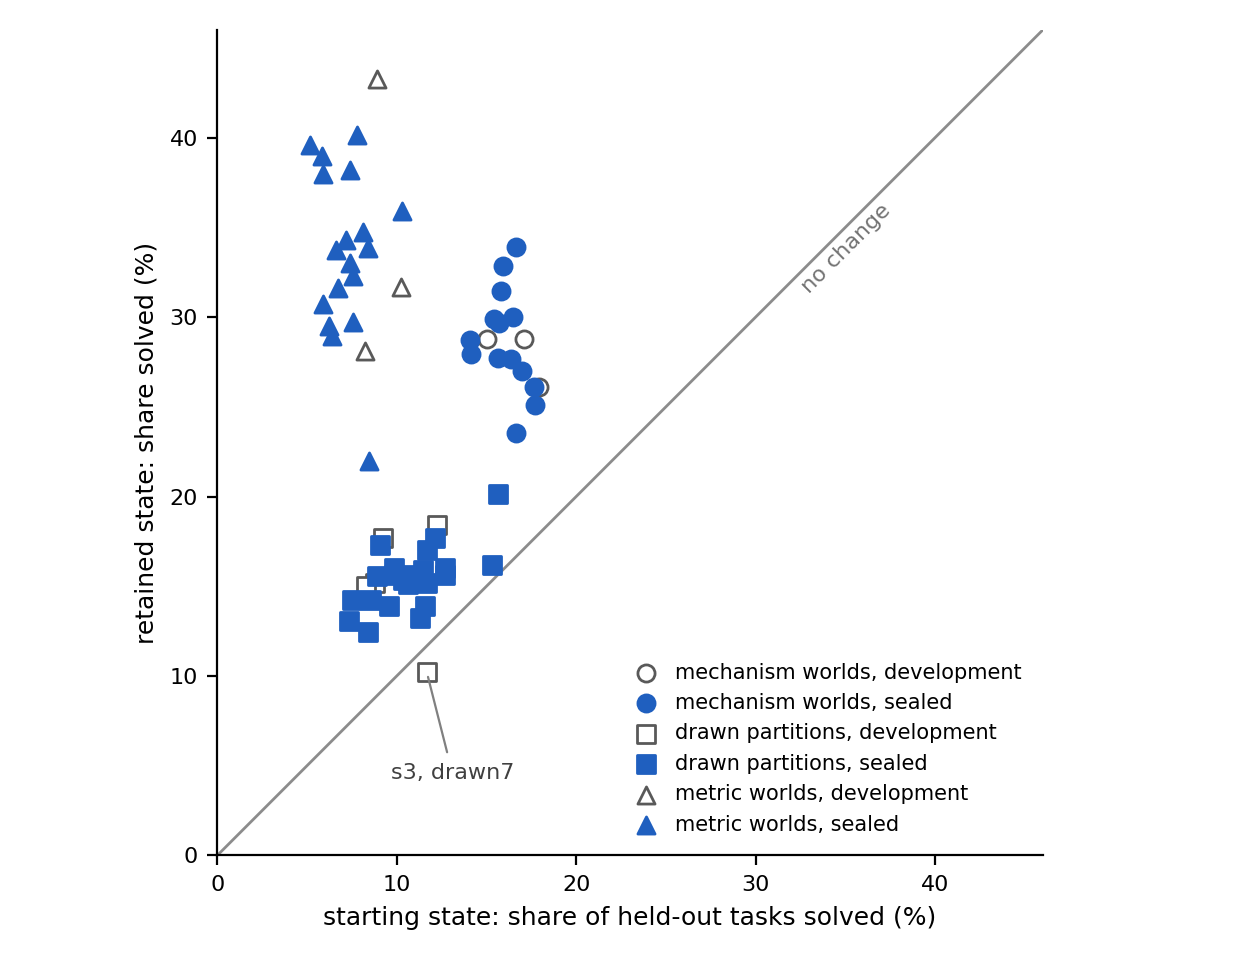
\includegraphics[width=0.88\linewidth]{fig-seed-growth.png}
\caption{Share of held-out tasks solved on sets no acceptance test used: the starting state (horizontal) against the retained state (vertical), one point per agent and area, 100 pairs in all (the three development agents in eleven, the nineteen sealed seeds in 89). A point above the diagonal improved. One pair fell, \texttt{s3} in the drawn partition.}
\label{fig:growth}
\end{figure}

\begin{table}[t]
\centering
\caption{Three-setting confirmation runs: tasks solved on fresh held-out sets (24 worlds per pool; 7,200, 2,400 and 4,800 tasks) by the starting and the retained state, the test-to-live cost ratio, and the gate outcome.}
\label{tab:confirm}
\footnotesize
\begin{tabular}{llllll}
\toprule
Seed (version) & mech & drawn7 & metric & cost & gates \\
\midrule
919100 (v1) & 1,128 to 1,997 & 236 to 385 & 405 to 1,055 & 5.96$\times$ & cost fails \\
919101 (v1) & 1,223 to 1,944 & 271 to 318 & 318 to 1,619 & 5.88$\times$ & cost fails \\
919102 (v2) & 1,020 to 2,010 & 281 to 409 & 364 to 1,550 & 1.89$\times$ & own-set clause fails \\
919103 (v2) & 1,200 to 1,697 & 255 to 363 & 363 to 1,428 & 1.98$\times$ & all pass \\
919104 (v3) & 1,276 to 1,807 & 280 to 364 & 373 to 1,927 & 2.29$\times$ & one stale baseline \\
919105 (v3) & 1,147 to 2,366 & 180 to 342 & 322 to 1,518 & 1.94$\times$ & one stale baseline \\
919106 (v4) & 1,129 to 2,136 & 202 to 299 & 343 to 1,647 & 2.32$\times$ & all pass \\
919107 (v4) & 1,138 to 2,263 & 275 to 382 & 248 to 1,901 & 2.04$\times$ & all pass \\
919108 (v5) & 1,179 to 1,990 & 367 to 388 & 281 to 1,872 & 2.48$\times$ & growth and safety fail \\
919109 (v5) & 1,111 to 2,151 & 278 to 334 & 404 to 1,626 & 2.53$\times$ & cost fails \\
\bottomrule
\end{tabular}
\end{table}

\begin{table}[t]
\centering
\caption{Six- and seven-setting confirmation runs (versions 6 to 10): tasks solved on fresh held-out sets (24 worlds per pool) by the starting and the retained state in each area, the test-to-live cost ratio, and the gate outcome. The cost gate was 2.5 for version 6, 3.25 for version 7 and 3.5 for versions 8 to 10.}
\label{tab:confirm6}
\footnotesize
\resizebox{\linewidth}{!}{%
\begin{tabular}{lllllllll}
\toprule
Seed (version) & mech & drawn7 & metric777001 & drawn11 & drawn13 & metric555001 & str7 & cost, gates \\
\midrule
919110 (v6) & 1,197 to 2,442 & 305 to 375 & 299 to 1,415 & 291 to 424 & 375 to 483 & 356 to 1,833 & -- & 2.78$\times$, cost fails \\
919111 (v6) & 1,187 to 2,160 & 305 to 384 & 355 to 1,585 & 206 to 341 & 176 to 314 & 283 to 1,475 & -- & 2.64$\times$, cost fails \\
919112 (v7) & 1,014 to 2,070 & 214 to 374 & 493 to 1,723 & 217 to 415 & 237 to 375 & 308 to 1,390 & -- & 2.88$\times$, all pass \\
919113 (v7) & 1,269 to 1,878 & 230 to 334 & 389 to 1,667 & 249 to 369 & 258 to 375 & 284 to 1,823 & -- & 2.32$\times$, all pass \\
919114 (v8) & 1,185 to 2,300 & 166 to 460 & 344 to 1,422 & 249 to 381 & 215 to 439 & 371 to 1,605 & 4,749 to 6,026 & 2.61$\times$, all pass \\
919115 (v8) & 1,174 to 1,885 & 320 to 413 & 309 to 1,409 & 251 to 386 & 322 to 430 & 300 to 1,321 & 4,119 to 5,419 & 2.71$\times$, all pass \\
919116 (v9) & 1,072 to 2,088 & 258 to 279 & 259 to 1,715 & 220 to 377 & 224 to 384 & 339 to 1,485 & 5,076 to 6,248 & 2.33$\times$, growth fails \\
919117 (v9) & 1,217 to 2,416 & 241 to 432 & 326 to 1,584 & 275 to 416 & 305 to 442 & 384 to 1,716 & 4,910 to 6,127 & 2.27$\times$, all pass \\
919118 (v10) & 1,159 to 2,484 & 273 to 349 & 450 to 2,283 & 241 to 439 & 286 to 379 & 378 to 1,329 & 4,722 to 6,193 & 2.92$\times$, all pass \\
\bottomrule
\end{tabular}}
\end{table}

\subsection{The totals across nineteen sealed seeds}

Every one of the 89 agent-and-area pairs of the sealed seeds improved on its fresh held-out set. Every one of the 171 accepted changes replayed exactly; the two stale baselines of version 3 were wrong recorded numbers, not wrong decisions, and nothing else was found. Growth of at least 15\% in every area held on seventeen seeds of nineteen; the two misses are seed 919108 under the retired guard and seed 919116's drawn partition at +8\%. No pool below 90\% of its start held on eighteen of nineteen; the one miss is 919108. Across the nine seeds that lived six or more areas, 59 of 59 area scores rose, by 8\% to 562\%, and 91 of 91 pools rose. The mechanism area's untrained pool, the one the development runs had flagged as the weak point, rose on seventeen of nineteen seeds to a median of 163\% of its start; its two dips, to 94\% on 919103 and 89\% on 919108, are both under early versions, and its outcome shows no relation to how many shared-language changes the other areas kept.

\section{What went wrong, and what each failure taught}

Each of the following was a real failure in the record. Each changed the design, and the design is best understood through them.

\subsection{A change in one area damaged another}
\label{sec:interference}

After four lives in metric worlds, the main agent's score on the first drawn partition's untouched held-out set had fallen from 376 to 338, a 10\% loss in an area it had not entered since. The cause was the shared language. The metric lives had accepted one extension of 40 atoms and one removal of 25, each tested on the metric area alone. A language that grew and shrank to suit metric worlds changed the catalog that the drawn partition's model had been fitted over. Each change was a tested success where it was tested and a regression where it was not.

The fix was the cross-area check of Section~\ref{sec:ops}: a language candidate is also run on a held-out set of every other area the agent has lived in and rejected if it falls more than 2\% behind there. The tolerance permits a small measured regression; it is a bound, not a guarantee of preservation. The check fired twice as soon as it existed. In \texttt{drawn11} a combination of invented atoms and a model gained 165 to 344 on that area's own held-out set and was rejected because it cost mechanism worlds 8\% and \texttt{drawn7} 12\%; the model alone was then accepted, at 417. In \texttt{drawn13} a combination worth 150 was rejected for costing \texttt{drawn11} 23\%. Each would have been accepted under the earlier rule. The \texttt{s3} case of Table~\ref{tab:growth} shows the check's remaining gap: a 12-world set read a gain where a 24-world set read a 12\% loss, which is why the confirmation protocol uses 24.

\subsection{The grown language diluted the search}
\label{sec:dilution}

At version 24 the main agent's untrained family combinations had fallen from 24 to 18 tasks per world on the mechanism area's untouched set, while trained worlds rose from 26 to 50. The acceptance tests had not noticed, because a test compares totals and the untrained pool is only a third of the set.

Table~\ref{tab:ablation} takes the retained state apart to find the cause. An \emph{ablation} removes one component at a time and measures what is lost. With the retained model and prior but the starting language, the state scores 1,973, with untrained combinations at 26 per world, above the start. With the grown language alone, no model and no prior, it scores 735 against 1,299 for the starting language. The 166 invented atoms then in the language, 110 of them behaviourally new, had enlarged the catalog from 82,758 rows to 266,272, and the half of each task's budget that the prior rule reserves for the no-prior order was scanning a catalog two thirds of which the agent had added. Trained worlds did not suffer, because the model's half of the budget found their rows anyway. Untrained combinations, which the model promotes less, did.

\begin{table}[t]
\centering
\caption{Ablation of \texttt{s1}'s retained state (version 24) on the mechanism area's untouched held-out set: tasks per world by pool, and total of 7,200.}
\label{tab:ablation}
\begin{tabular}{lrrrr}
\toprule
State & Trained & Unfamiliar & Untrained & Total \\
\midrule
retained & 49.5 & 18.7 & 18.2 & 2,072 \\
retained, no prior & 43.0 & 14.7 & 9.5 & 1,614 \\
retained, no model & 37.3 & 15.0 & 15.9 & 1,639 \\
grown language only, no model, no prior & 11.1 & 9.0 & 10.5 & 735 \\
starting language, retained model and prior & 50.0 & 6.1 & 26.2 & 1,973 \\
starting state & 26.2 & 3.7 & 24.2 & 1,299 \\
\bottomrule
\end{tabular}
\end{table}

The agent already held the verdict it needed. Its self model files an atom in no group when the agent would almost never find it in a world. Across the five area models, 107 invented atoms were rated real by at least one model, 55 of the 56 that reproduce a withheld family among them, and 59 were rated import-only by every model that had seen them, one of them real. From version 26 the prune operation proposes those too, and the acceptance test decides. On life 11 the removal of 55 atoms was accepted, and the model and extension proposed beside it were rejected on intervals that crossed zero. The language went from 426 to 371 atoms, and untrained combinations recovered to 18.6 against a start of 20.5, with every other pool and area above its start.

Two further revisions went in at the same version. First, the acceptance rule had been ``solve strictly more tasks than the current state'', and on life 10 a model was accepted for a gain of 24 tasks on 72 worlds that read 82 \emph{lower} on the untouched set; the bootstrap interval replaced the strict inequality. Second, the tie-break, the order the scan uses among rows it scores equally, had been a random shuffle of row positions, so adding or removing any atom reshuffled every other row and every language test carried that noise. It is now a fingerprint of each row's content, so a language change changes nothing but the rows it adds or removes.

\subsection{A gate missed at its own noise level}
\label{sec:noise}

Seed 919116 under version 9 failed the growth gate in \texttt{drawn7} at +8\% against the required 15\%. The question was whether something had gone wrong or whether the check was too noisy to tell. Replaying that area's fresh 24-world set with the state after each accepted change answered it: the score stood at 258 at the start, 283 after the area's own accepted change (+10\%), and between 259 and 283 under every later shared-language change, ending at 279. Not cumulative drift: one accepted change whose gain on its 48-world test set (+35\%) generalised to +10\% on the fresh set, after which the area's later candidates, at +7\% to +10\% on 48 worlds, were rejected because their intervals included zero.

The acceptance test can detect a 15\% gain in a single-pool area on 48 worlds only barely. Version 10's extension set is the response: a candidate that lands near the threshold gets a second sample of the same size before it is rejected, and the decision uses both.

\subsection{Smaller things}

\paragraph{The test cost six times the living.} Version 1's remedy was structural: longer lives, held-out sets reused until something is accepted on them, and stopping a losing candidate at the half set.

\paragraph{Two bookkeeping flaws.} Two parts of one life accepted on the same set (version 2), and a cached baseline that went stale as experience grew (version 3). Neither changed a decision. Both were caught only because the audit replays everything.

\paragraph{A guard that could not do its job.} Version 5's per-candidate tolerance on unguided search let three candidates, each inside tolerance, add up to an 11\% dip. A later check across all nineteen seeds found no cumulative drift in the pool the guard was meant to protect, so no replacement guard was added.

\paragraph{A filter that excluded the right answers.} The string worker's consistency test rejected pieces that the puzzle generator itself uses. A tenth of the tasks were unsolvable in principle until version 9.

\paragraph{The host machine.} One stall, one crash and one interrupted run in the record were the machine's memory, not the agent.

\section{What this does and does not show}
\label{sec:shows}

It shows one program improving its own state in seven settings of different structure, across two kinds of puzzle, keeping only changes that it tested on worlds it never trained on, with every test charged and every acceptance independently replayed. The three forms of growth from the earlier work appear together in its ledger: within-life accumulation in every life, learned search guidance accepted nearly every life and accounting for most of the measured gain, and invented atoms that let it reach families its starting language could not express. Growth in one area did not require starting over in another; the language carried, and in two six-area runs an area that kept no change of its own still rose more than fourfold from what the other areas had built.

It is improvement of state, not of procedure. The agent's model and language direct its search, its search produces the experience the next model and language are fitted from, and the ledger shows the state improving the state across many lives. But the procedures that turn experience into a model, candidates into atoms, and tests into acceptances are fixed code, and every revision of the acceptance rule was made by the experimenter. A later agent does not produce a better reflect or a better extend. By this programme's definition, recursive self-improvement is not met.

The growth also saturates and is uneven. On the main agent's later mechanism lives few candidates passed, and model gains fell from hundreds of tasks to single digits by the sixth life. Half of the remaining invented atoms are behaviourally new and some are surely junk that costs budget until a removal takes them out. Testing costs two to three times living. The two puzzle forms are both small and synthetic, and no setting involves a real-world domain.

The held-out sets behind the tables are single draws whose per-world results were not saved, so no interval accompanies the totals; the figure's points are totals only. Two accepted changes of a development agent's run do not replay, for a reason not found.

\section{Lessons}

\begin{enumerate}[leftmargin=*]
\item The acceptance test is the design. Every choice that mattered concerned what counts as an accepted change: a paired interval above zero on a fresh held-out set, within tolerance everywhere the state is shared, cost charged. Given that rule, a weak candidate costs a test and nothing else, so the agent can propose freely.
\item Test the combination first, then the parts. This halved the tests in the common case and lost nothing.
\item Invention needs recurrence. An atom that fits one uncovered task is usually a coincidence; one that fits two is usually a missing atom.
\item Let the agent remove what it added. Removals were accepted whenever proposed, and removing the atoms the self model called import-only recovered a loss no test had seen.
\item Shared state needs shared tests. The 10\% loss in an untouched area was invisible to any single-area test.
\item Score growth on worlds the agent never saw, and attach an interval. A gain of 24 on 72 worlds is noise.
\item Make the measurement stable under the change being measured. A tie-break over row positions turned every language change into a reshuffle of the whole catalog.
\item A gate at the noise level of its check will fail by chance. Give borderline candidates a second sample before rejecting them.
\item Freeze, seal, forecast, replay. Every flaw found in the confirmation phase was found by the audit, and none would have been found by looking at the scores.
\end{enumerate}

\section{What comes next}

\begin{itemize}[leftmargin=*]
\item The clean rerun of seed 919119 under version 10, then the version 10 verdict.
\item An eighth setting: a second string-task area with a different split of trained and untrained key families, already smoke-tested with no new code. Version 11 would add it with three lives, 24 lives over eight areas, and a cost gate of 3.75, to be frozen only after the version 10 verdict.
\item Intervals on the reported gains, by saving per-world results in the final checks.
\item The next level: letting the agent improve a procedure, not just its state. The first candidate is the acceptance test itself, learning from its ledger how large a held-out set each kind of change needs.
\end{itemize}

\section{Glossary}

\begin{description}[leftmargin=*,style=nextline]
\item[Acceptance test (``prove'')] The comparison that decides whether a proposed change is kept: both states run on the same held-out worlds, and the change is accepted only if the 95\% bootstrap interval of its per-world gain lies above zero and, for a language change, it stays within 2\% on every other lived area of the same form.
\item[Area] A recipe for generating worlds with a particular hidden structure. Seven are used: mechanism worlds, three drawn partitions, two metric weightings and string tasks.
\item[Atom] One simple yes-or-no rule about a character, the smallest building block. 313 exist in 9 families; the agent starts with 260.
\item[Audit] An independent replay of every accepted change from saved state, checking that the recorded totals and interval come out identical.
\item[Bootstrap interval] A range estimated by resampling the observed per-world differences with replacement many times (4,000 here) and taking the middle 95\% of the resampled averages. If it lies entirely above zero, the gain is unlikely to be luck.
\item[Carried state] Everything the agent keeps between lives: language, experience, per-area model and prior, invented atoms, ledger and resource account.
\item[Catalog] Every candidate rule the current language can build, one row per distinct behaviour. 82,758 rows from the starting language.
\item[Confident pick] A submission made when exactly one consistent rule lay in the scanned window. Right about 90\% of the time; not a guarantee.
\item[Cross-area check] The part of the acceptance test that runs a language change on a held-out set of every other lived area of the same form and rejects it if it falls more than 2\% behind there.
\item[Discovery rate] How often the agent finds an atom when a world contains it, as estimated by its own model. An atom below 0.10 is filed in no group.
\item[Earned experience] The atoms behind the agent's own submissions in a world, kept whether the submission was right or wrong.
\item[Extension set] A second held-out set of the same size, drawn fresh, on which a candidate near the acceptance threshold is run before the decision is made on both sets together. Added in version 10.
\item[Family] One of 9 kinds of atom, named for its arithmetic operation. Two families, popcount and xormod, are withheld from the starting language.
\item[Gate] A pass-or-fail condition stated before a confirmation run. The four are growth (every area up at least 15\%), safety (no pool below 90\% of its start), cost (testing at most a stated multiple of living) and audit (every acceptance replays exactly, on its own set).
\item[Hash] A short fingerprint computed from a file's exact contents. The frozen protocol records the hashes of the source files.
\item[Held-out set] Worlds the agent never lived, used only to compare two states. Fresh held-out sets, drawn with a salt no test used, give the reported gains.
\item[Import rate] How often the agent earns an atom through a wrong pick in a world that does not contain it, as estimated by its own model.
\item[Language] The set of atoms the agent currently holds. Not a natural language.
\item[Life] One round of experience (48 or 96 worlds of one area, 100 tasks each) followed by proposing and testing changes.
\item[Paired comparison] Comparing two states on the same worlds and recording the per-world difference, so that variation in world difficulty cancels.
\item[Pool] A subset of an area's worlds that the scoring can tell apart but the agent cannot: trained, untrained and unfamiliar in mechanism worlds and string tasks.
\item[Prior (search prior)] A starting order for the catalog based on how often atoms appeared together in the agent's own earlier worlds of an area. Half of each task's budget is reserved for the order the agent would use without it.
\item[Random seed] A number that fixes every pseudorandom choice a run makes, so the run can be repeated exactly. Sealed seeds were chosen in advance and never used before.
\item[Replay] Rebuilding the state before and after an accepted change and running the same test again. ``Replays exactly'' means the totals and interval match the ledger.
\item[Salt] An extra number mixed into a random draw so that one held-out set differs from every other.
\item[Scan] Looking at one candidate rule. The budget is 1,024 scans per task.
\item[Seed agent] The program plus its carried state. The thing that grows.
\item[State and procedure] State is what the program carries and changes; procedure is the fixed code that reads and writes it. This work improves state only.
\item[Task] One puzzle: a hidden rule, eight visible examples (three in the string form) and sixteen hidden ones (six in the string form).
\item[Tie-break] The order the scan uses among catalog rows it scores equally. Now a fingerprint of each row's content, so that a language change does not reshuffle unrelated rows.
\item[World] A hidden set of 14 atoms and 100 tasks whose rules are built only from them.
\item[World and self model] An area's fitted model of which atoms occur together (world) and how reliably the agent finds each (self). It guides search and supplies the import-only verdict that prune uses.
\end{description}

\section{Reproducibility}

The technical companion to this paper, with the same results in the field's own terms, is \path{paper/seed-growth.tex} in the RSI repository at \path{projects/rsi}; a living copy is at \url{https://claude.ai/code/artifact/ebd48ba7-84b1-4bb2-b2e5-eb18375651bc}. The seed agent is \path{rsi/seed.py} (state, areas, the operations and the acceptance test) and \path{rsi/seed_string.py} (the string-task form), with \path{rsi/seed_areas.py} for metric worlds, \path{rsi/invention.py} for the grammar and the recurrence test, and \path{rsi/self_world_model.py} for the model. \path{seed_run.py} runs lives and resumes from saved state; \path{seed_check.py} scores an agent on fresh held-out sets; \path{audit_seed.py} replays accepted changes from version snapshots; \path{confirm_seed.sh <name> <seed>} runs the frozen confirmation schedule, check and audit described in \path{EXPERIMENT-seed-confirmation.md}, whose nineteen runs are in \path{seeds/c1} to \path{seeds/c19}. States are in \path{seeds/<name>/state.json}; the ledger inside each is the full record of every candidate, its test and its cost. The worked task of Section~\ref{sec:puzzles} is reproduced by drawing the first trained world of \path{MechanismArea(644101)} with \path{random.Random(7)} and the task from its first mechanism with \path{random.Random(11)}.

Settings: 48 worlds of 100 tasks per life in development and 96 in confirmation; budget 1,024 scans per task; held-out sets of 24 worlds per pool in development and at least 48 in confirmation, cross-area sets of 12 and 24; tolerance 2\% relative; 6 to 8 groups and 2 to 4 groups per world by held-out likelihood; extension cap 40 atoms per life with recurrence 2; removal after 2 lives or on the self model's import-only verdict; tie-break a content hash per row with seed 77; a change accepted only when the paired 95\% bootstrap interval (4,000 draws) of its gain is above zero, or, from version 10, when the interval over the proof set and one extension set is.

\end{document}
